\documentclass[14pt, a4paper]{report}
\usepackage{mathtext}
\usepackage[T2A]{fontenc}
\usepackage[utf8]{inputenc}
\usepackage[russian]{babel}
\usepackage{multirow}
\usepackage{graphicx}
\renewcommand{\thesection}{\arabic{section}.}

\title{\textbf{Отчет о выполнении лабораторной работы 1.3.3 "Измерение вязкости воздуха по течению в тонких трубках"}}
\author{Калашников Михаил, Б03-205}
\date{}

\begin{document}
\maketitle

\textbf{Цель работы:}
экспериментально исследовать свойства течения газов по тонким трубкам при различных числах Рейнольдса; выявить область применимости закона Пуазейля и с его помощью определить коэффициент вязкости воздуха.
\newline

\textbf{В работе используются:}
\begin{itemize}
\item система подачи воздуха (компрессор, поводящие трубки); 
\item газовый счетчик барабанного типа ($\sigma_V=0,02\ л$);
\item спиртовой микроманометр с регулируемым наклоном ($\rho=0,8095\pm0.0005\ г/см^3$, $\sigma_h=1\ мм$);
\item набор трубок различного диаметра с выходами для подсоединения микроманометра ($d_1=3,0\pm0,1\ мм$, $d_2=3,95\pm0,05\ мм$, $d_3=5,05\pm0,05\ мм$);
\item секундомер
\end{itemize}

\section{Теоретическая часть}
Сила вязкого трения как в жидкостях, так и в газах описывается законом
Ньютона: касательное напряжение между слоями пропорционально перепаду
скорости течения в направлении, поперечном к потоку:
\[\tau_z = -\eta \frac{\delta \upsilon_x}{\delta y}\]
\paragraph{}
Характер течения определяется безразмерным параметром задачи — числом Рейнольдса:
\[Re =  \frac{\rho u a}{\eta}\]
\paragraph{Течение Пуазейля.} Из опыта известно, что при достаточно малых числах
Рейнольдса течение в прямой трубе с гладкими стенками имеет ламинарный
характер. В таком случае будет верна формула Пуазеля, которая позволяет найти вязкость газа по зависимости расхода от перепада давления в трубе и используется в качестве основной расчётной формулы в данной работе:
\[Q = \frac{\pi R^{4} \Delta P}{8 \eta l}\]	
\paragraph{Длина установления.} Пусть на вход трубы поступает течение, распределение скоростей которого не является пуазейлевским. Профиль течения не может установиться сразу, а реализуется лишь на некотором расстоянии $l_{уст}$ от начала трубы. Грубая оценка для этой величины, с учётом экспериментально установленного коэффициента, позволяющего добиться удовлетворительной точности:
\[l_{уст} \sim \frac{\rho u R^{2} }{\eta} \approx 0,2 R \cdot Re\]
\paragraph{Турбулентность.} Ламинарная картина течения наблюдается при относительно малых числах Рейнольдса, когда вязкие силы достаточны для того,
чтобы погасить любые случайно возникшие возмущения потока. При превышении некоторого критического числа Рейнольдса Re > Re.кр течение Пуазейля становится неустойчивым. В потоке начинают рождаться вихри, которые затем сносятся вниз по трубе (при докритических числах Рейнольдса такие вихри быстро затухают за счёт вязкости). С дальнейшим увеличением Re
количество вихрей возрастает и, взаимодействуя между собой, они порождают вихри всё меньшего размера, создавая таким образом сложную многомасштабную картин течения. Эта картина радикально отличается от ламинарной: в ней отсутствуют непрерывные
линии тока, а слои жидкости постоянно перемешиваются. Течение становится практически непредсказуемым, а скорость и давление испытывают значительные случайные флуктуации. В таком потоке расход можно оценить следующим образом:
\[Q\sim R^\frac{5}{2}\sqrt{\frac{\Delta P}{\rho l}}\]

\section{Экспериментальная установка}

\begin{figure}[!ht]
\centering
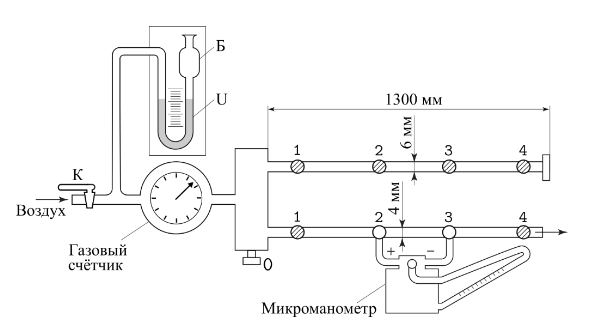
\includegraphics[width=0.6\linewidth]{terma3_0.png}
\caption{Экспериментальная установка}
\end{figure}

Поток воздуха под давлением, немного превышающим атмосферное, поступает через газовый счётчик в тонкие металлические трубки. Воздух нагнетается компрессором, интенсивность его подачи регулируется краном К. Трубки снабжены съёмными заглушками на концах и рядом миллиметровых отверстий, к которым можно подключать микроманометр. В рабочем состоянии открыта заглушка на одной (рабочей) трубке, микроманометр подключён к двум её выводам, а все остальные отверстия плотно закрыты пробками. Перед входом в газовый счётчик установлен водяной U-образный манометр. Он служит для измерения давления газа на входе, а также предохраняет счётчик от выхода из строя. 

\section{Проведение эксперимента}

\begin{enumerate}

\item Перед началом работы ознакомимся с характеристиком установки и измерительных приборов.

\item Подсоединим манометр к двум соседним выводам трубки среднего диаметра ($l=50\ см$). Включим компрессор и создадим поток воздуха через трубку, следя за показаниями микроманометра. Убедимся в работоспособности установки.

\item Измерим параметры окружающей среды: $t_0=23,7 ^\circ C$, $\rho_0=20,9\%$, $P_0=97,59\ кПа$. Из таблицы определим поправочный коэффициент к плотности спирта: $k=0,9932$. Зафиксируем диаметры трубок.

\item Рассчитаем критическое значение расхода.
\[Re=\frac{\rho ua}{\eta}\approx\frac{\rho Qa}{\pi R^2\eta}\approx\frac{\rho Q}{\pi R\eta}=\frac{\mu P_0Q}{R_гT_0\pi R\eta}\]
\[Q_{кр}=\frac{R_гT_0\pi R\eta Re_{кр}}{\mu P_0}\approx6,5\ л/мин\]

Далее выразим соответвующий данному расходу перепад давлений.
\[Q=\frac{\pi R^4\Delta P}{8\eta l}\]
\[\Delta P_{кр}=\frac{8\eta lQ_{кр}}{\pi R^4}\approx180\ Па\]
Переведя это в деления шкалы микроманометра, получим 114 мм.

Оценим длину, на которой течение можно считать установившимся.
\[l_{уст}=0,2Re_{кр}R\approx40\ см\]
Расстояние от начала трубки до ближайшего вывода, подключенного к микроманометру превышает 80 см, то есть течение можно с уверенностью считать установившимся.

\item Визуально определим границу перехода от ламинарного течения к турбулентному. Столбик микроманометра начинает заметно колебаться при превышении отметки в 80 мм. Данная величина немного ниже чем оценка, полученная в предыдущем пункте.

\item Найдем параметры расхода, при которых относительная погрешность не будет превышать 1\%.
Так как $\sigma_V=0,02\ л$, то минимальный объём проходящего через счётчик газа нужно принять равным 2 литрам. Проведя простые измерения скорости реакции человека с помощью секундомера, мы определили, что она не превышает $\sigma_t=0,2\ с$. Так как, мы фиксируем время начала и конца процесса измерения, абсолютная погрешность удваивается. То есть минимальное время измерения должно превышать 40 с.

\item Измерим зависимость перепада давления $\Delta P$ от расхода $Q$ на выбраном участке. Проведем пять измерения в ламинарном режиме течения, пять -- в турбулентном и еще две в зоне, находящейся в промежуточной зоне. Результаты запишем в таблицу 1. Обработаем их, вычислив $\Delta P$ и $Q$ по формулам:
\[\Delta P=\rho_с kgh \sin\alpha,\quad Q=\frac{V}{t}\]
где $\rho_с$ -- плотность спирта, $k$ -- поправочный температурный коэффициент, $g$ -- ускорение свободного падения, $\sin\alpha=0,2$ на протяжении всей лабораторной работы. Обработанные результаты занесем в таблицу 2.

\item Проведем измерение распределения давления газа вдоль трубки. Подсоединим микроманометр ко всевозможным парам отверстий. Результаты занесем в таблицу 3.

\item Повторим предыдущие пять пунктов для трубки с наибольшим диаметром. Дополним таблицы 1-3.

\item Измерим зависимость расхода от радиуса трубы при заданном градиенте давления. Измерим расход всех труб, при градиенте, обеспечивающем ламинарное течение, и при градиенте, обеспечивающем турбулентное течение. Заполним получившимися данными таблицу 4.

\end{enumerate}

\section{Обработка данных}

\begin{enumerate}

\setcounter{enumi}{10}

\item По данным таблицы 2 построим графики зависимости $Q(\Delta P)$. На графиках отчетливо видна граница перехода от ламинарного режима течения, к турбулентному. По угловым коэффициентам линейных зависимостей для ламинарных потоков определим вязкость воздуха.
\[Q=\frac{\pi R^4\Delta P}{8\eta l}=k\Delta P,\]
\[k=\frac{\pi R^4}{8\eta l},\quad \eta=\frac{\pi R^4}{8kl}\]
Также рассчитаем критическое число Рейнольдса по формуле из пункта 4:
\[Re_{кр}=\frac{\mu P_0Q_{кр}}{R_гT_0\pi R\eta}\]
\[Re_1=1010,\quad Re_2=1220\]

\item Построим график зависимости $\Delta P(x)$, используя данные из таблицы 3. За ноль примем давление на выходе из трубки. Оценим длину установления $l_{уст}$ и отметим ее на графике. Действительно, после пересечения $l_{уст}$ давление газа меняется линейным образом.

\item Теперь построим график зависимости $\ln Q(\ln R)$, основываясь на данных из таблицы 4. Угловой коэффициент данной прямой будет равен показателю степени $\beta$ в зависимости $Q\propto R^\beta$. Как можно заметить из графика (рисунок 4) точка, соответствующая трубе наименьшего диаметра очень плохо ложится на прямую. Исключив ее, можно найти $\beta$ по двум оставшимся точкам.

\[\beta_1=4,6,\quad \beta_2=3,2\]

\end{enumerate}

\section{Расчет погрешностей}

Определим погрешность всех измеренных и вычисленных значений.
\[\varepsilon_{\Delta P}\approx\varepsilon_h=<\frac{\sigma_h}{h}>=4,2\%\ (\varepsilon_{\rho_с}\ll\varepsilon_h)\]
\[\varepsilon_Q=\sqrt{\varepsilon_{\Delta P}^2+\varepsilon_{t}^2}=0,9\%\]

Найдем погрешность вязкости воздуха $\eta$.
\[\varepsilon_{\eta,\ случ}=\varepsilon_{k}, \quad \varepsilon_{\eta,\ инст}=4\varepsilon_R\]
\[\varepsilon_{\eta}=\sqrt{\varepsilon_{\eta,\ случ}^2 + \varepsilon_{\eta,\ инст}^2}=\sqrt{\varepsilon_{k}^2 + 16\varepsilon_R^2}\]
\[\varepsilon_{\eta_1}=6,1\%\quad\varepsilon_{\eta_2}=6,2\%\]
\[\eta_1=17,0\pm1,0\ мкПа\cdot с,\quad\eta_2=14,9\pm0,9\ мкПа\cdot с\]

\section{Вывод}

Полученные значения вязкости близки с табличным значением, равным $17,8\ мкПа\cdot с$.

Показатели степени $\beta_1$ и $\beta_2$ полученные из теоритических зависимостей должны быть равны 4 и 2,5 соответственно. Значения, полученные из опыта довольно сильно отличаются.

\section{Приложения}

\begin{table}[!ht]
\centering
\begin{tabular}{| c | c | c | c | c | c |}
\hline
\multicolumn{3}{| c |}{$d=3,95\ мм$} & \multicolumn{3}{| c |}{$d=5,05\ мм$} \\
\hline
$h,\ мм$ & $V,\ л$ & $t, с$ & $h,\ мм$ & $V,\ л$ & $t, с$ \\
\hline
5	 & 0,4	 & 01:23,99	 & 5	 & 1,5	 & 00:54,97 \\
10	 & 0,5	 & 00:39,48	 & 11	 & 2,5	 & 00:49,47 \\
20	 & 1,0	 & 00:43,26	 & 14	 & 2,5	 & 00:41,04 \\
25	 & 1,5	 & 00:51,02	 & 22	 & 4,0	 & 00:42,88 \\
30	 & 1,5	 & 00:43,04	 & 28	 & 5,0	 & 00:44,30 \\
35	 & 2,0	 & 00:45,70	 & 31	 & 5,0	 & 00:41,10 \\
40	 & 3,0	 & 01:00,05	 & 39	 & 6,0	 & 00:43,30 \\
45	 & 3,0	 & 00:54,62	 & 53	 & 6,5	 & 00:45,58 \\
65	 & 4,0	 & 00:50:42	 & 56	 & 6,5	 & 00:42,10 \\
80	 & 4,5	 & 00:48:87	 & 61	 & 7,0	 & 00:42,60 \\
90	 & 5,0	 & 00:51,99	 & 92	 & 10,0	 & 00:51,73 \\
120	 & 4,5	 & 00:42,45	 & 102	 & 10,0	 & 00:48,35 \\
150	 & 5,0	 & 00:42,69	 & 	 & 	 & \\
165	 & 5,5	 & 00:45,25	 & 	 & 	 & \\
260	 & 6,0	 & 00:38,97	 & 	 & 	 & \\
\hline
\end{tabular}
\caption{Измерения расхода воздуха в зависимости от перепада давления}
\end{table}

\begin{table}[!ht]
\centering
\begin{tabular}{| c | c | c | c |}
\hline
\multicolumn{2}{| c |}{$d=3,95\ мм$} & \multicolumn{2}{| c |}{$d=5,05\ мм$} \\
\hline
$\Delta P,\ Па$ & $Q,\ л/мин$ & $\Delta P,\ Па$ & $Q,\ л/мин$ \\
\hline
7,9		& 0,29	& 7,9	& 1,64 \\
15,9	& 0,76	& 17,3	& 3,03 \\
31,8	& 1,39	& 22,1	& 3,66 \\
39,7	& 1,76	& 34,7	& 5,60 \\
47,6		& 2,09	& 44,2	& 6,77 \\
55,6	& 2,63	& 48,9	& 7,30 \\
63,5	& 3,00	& 61,5	& 8,31 \\
71,4	& 3,30	& 83,6	& 8,56 \\
103,2	& 4,76	& 88,3	& 9,26 \\
127,0	& 5,53	& 96,2	& 9,86 \\
142,9	& 5,77	& 145,1& 11,60 \\
190,5	& 6,36	& 160,8& 12,41 \\
238,3	& 7,03 & & \\
262,0	& 7,29 & & \\
412,8	& 9,24 & & \\ 
\hline
\end{tabular}
\caption{Зависимость расхода воздуха от перепада давления}
\end{table}

\begin{table}[!ht]
\centering
\begin{tabular}{| c | c | c | c | c | c | c | c | c | c | c |}
\cline{1-5}
\cline{7-11}
\multicolumn{5}{| c |}{$d=3,95\ мм$} & & \multicolumn{5}{| c |}{$d=5,05\ мм$} \\
\cline{1-5}
\cline{7-11}
$N$	& \multicolumn{1}{c}{1} & \multicolumn{1}{c}{2} & \multicolumn{1}{c}{3} & 4 & & $N$ & \multicolumn{1}{c}{1} & \multicolumn{1}{c}{2} & \multicolumn{1}{c}{3} & 4 \\
\cline{1-5}
\cline{7-11}
$1$ & \multicolumn{1}{c}{-} & \multicolumn{1}{c}{73}& \multicolumn{1}{c}{122} & 180 & & $1$ & \multicolumn{1}{c}{-} & \multicolumn{1}{c}{18} & \multicolumn{1}{c}{47} & 74 \\
$2$ & \multicolumn{1}{c}{-} & \multicolumn{1}{c}{-} & \multicolumn{1}{c}{48} & 108 & & $2$ & \multicolumn{1}{c}{-} & \multicolumn{1}{c}{-} & \multicolumn{1}{c}{29} & 55 \\
$3$ & \multicolumn{1}{c}{-} & \multicolumn{1}{c}{-} & \multicolumn{1}{c}{-} & 60  & & $3$ & \multicolumn{1}{c}{-} & \multicolumn{1}{c}{-} &  \multicolumn{1}{c}{-} & 27 \\
$4$ & \multicolumn{1}{c}{-} & \multicolumn{1}{c}{-} & \multicolumn{1}{c}{-} & - & & $4$ & \multicolumn{1}{c}{-} & \multicolumn{1}{c}{-} & \multicolumn{1}{c}{-} & - \\
\cline{1-5}
\cline{7-11}
$x,\ см$ & \multicolumn{1}{c}{11,5} & \multicolumn{1}{c}{41,5} & \multicolumn{1}{c}{81,5} & 131,5 & & $x,\ см$ & \multicolumn{1}{c}{11,5} & \multicolumn{1}{c}{41,5} & \multicolumn{1}{c}{81,5} & 131,5 \\
\cline{1-5}
\cline{7-11}
\end{tabular}
\caption{Измерение давления между всевозможными парами выводов, мм столбца микроманометра}
\end{table}

\begin{table}[!ht]
\centering
\begin{tabular}{| c | c | c | c | c | c | c |}
\hline
$\Delta h/\Delta l$ & \multicolumn{3}{| c |}{0.5 мм/см} & \multicolumn{3}{| c |}{3.6 мм/см} \\
\hline
$d,\ мм$ & $V,\ л$ & $t, с$ & $Q,\ л/мин$ & $V,\ л$ & $t, с$ & $Q,\ л/мин$ \\
\hline
3,0 & 1,2 & 00:45,20 & 1,593 & 6,0 & 00:36,51 & 5,930 \\
3,95 & 1,5 & 00:51,69 & 1,741 & 6,0 & 00:48,44 & 7,432 \\
5,05 & 4,0 & 00:44,15 & 5,436 & 10,0 & 01:00,71 & 16,389 \\
\hline
\end{tabular}
\caption{Измерение зависимости $Q(R)$ при ламинарном и турбулентном режимах течения}
\end{table}

\begin{figure}[!ht]
\centering
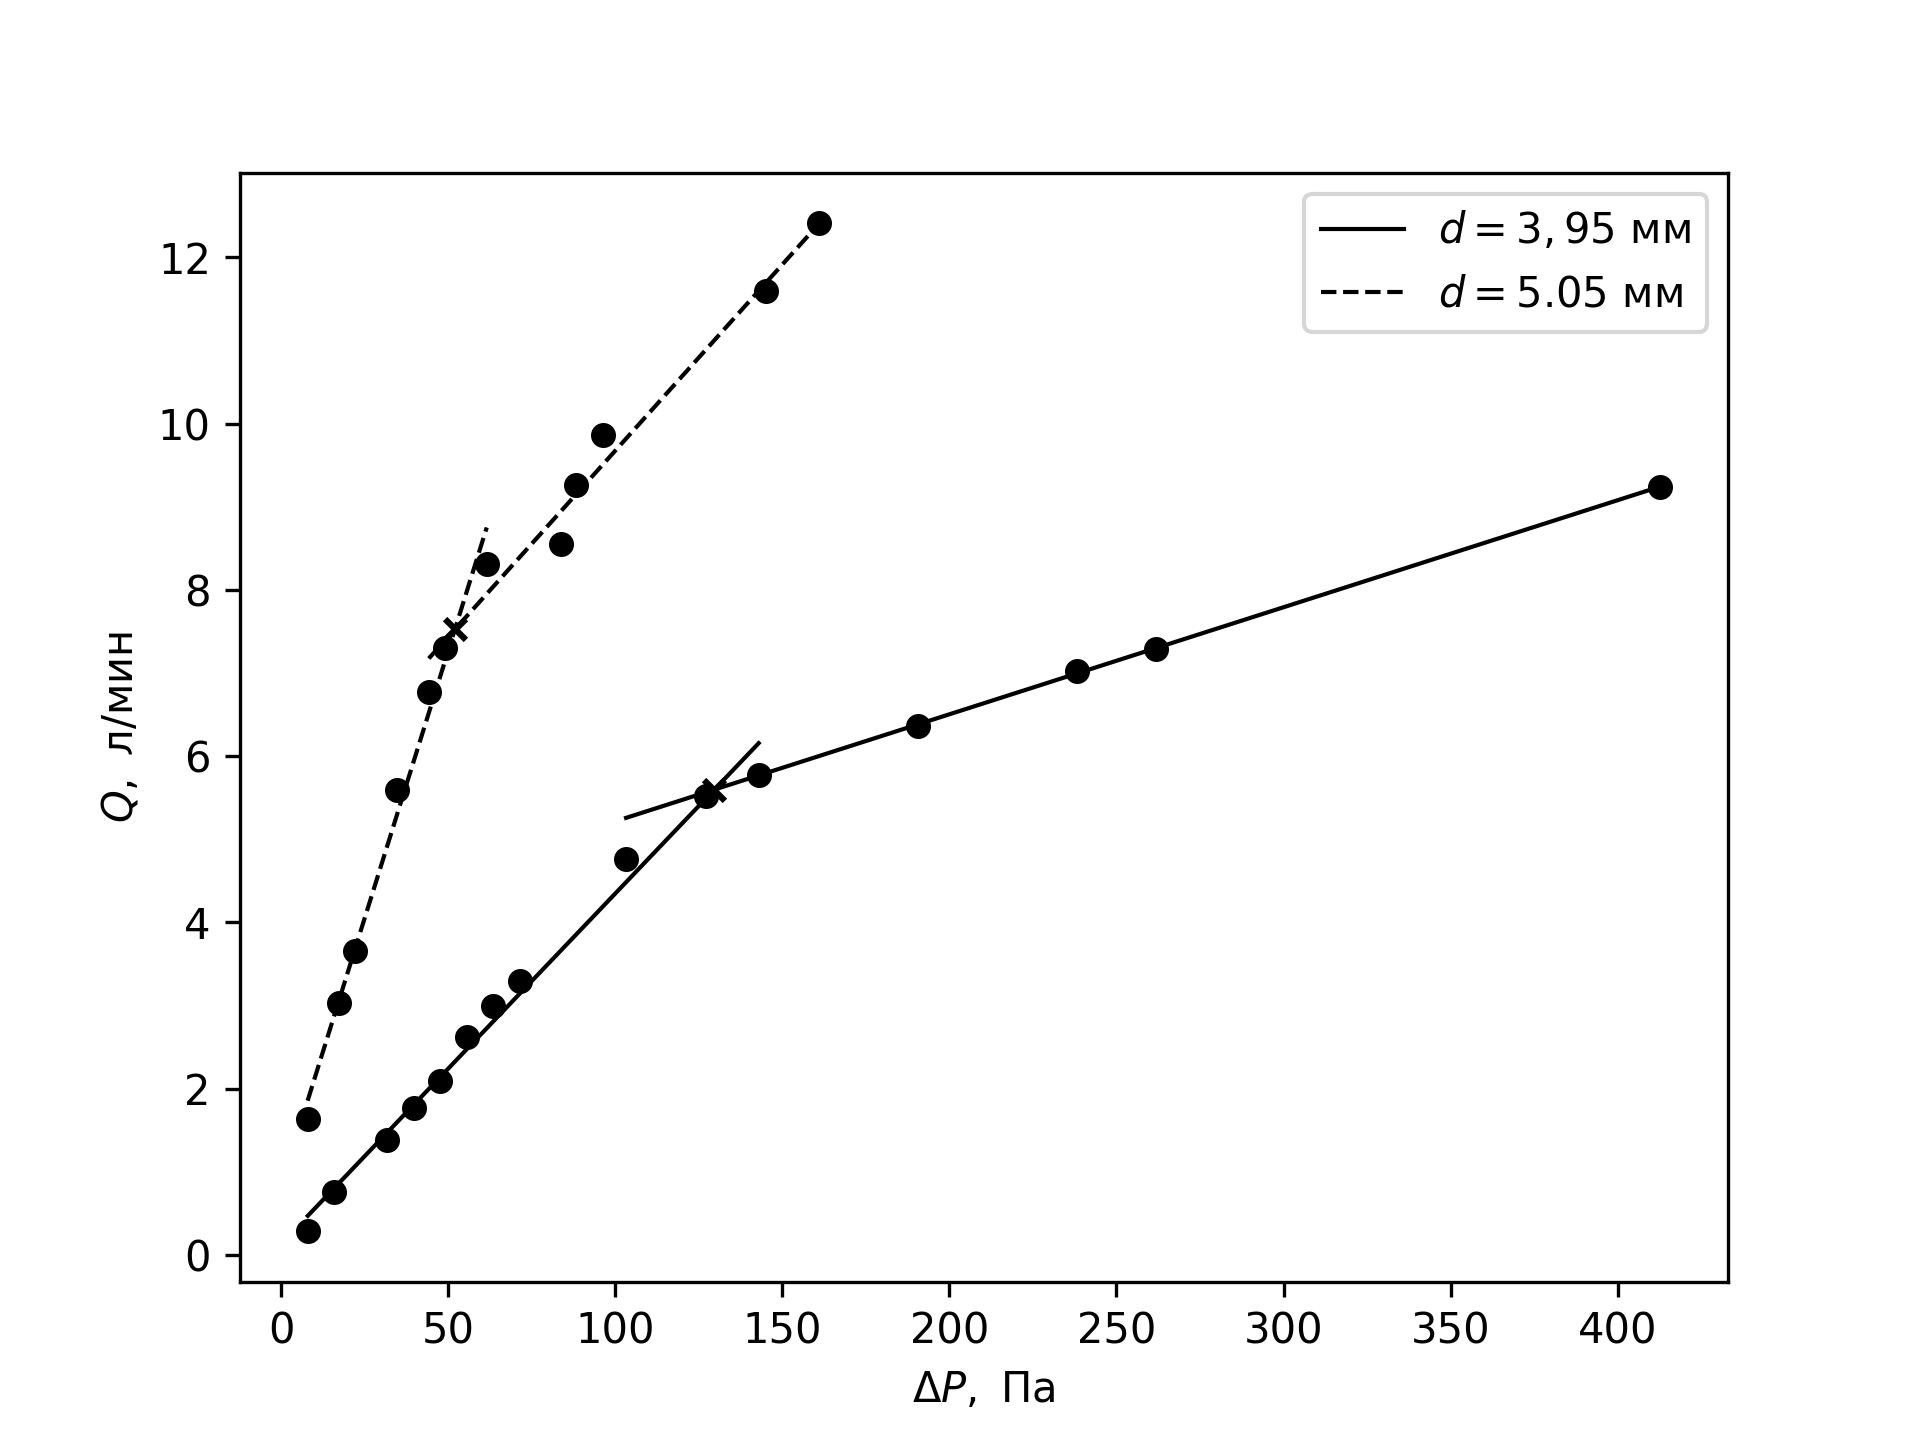
\includegraphics[width=0.8\linewidth]{terma3_1.png}
\caption{Зависимость расхода воздуха от перепада давления}
\end{figure}

\begin{figure}[!ht]
\centering
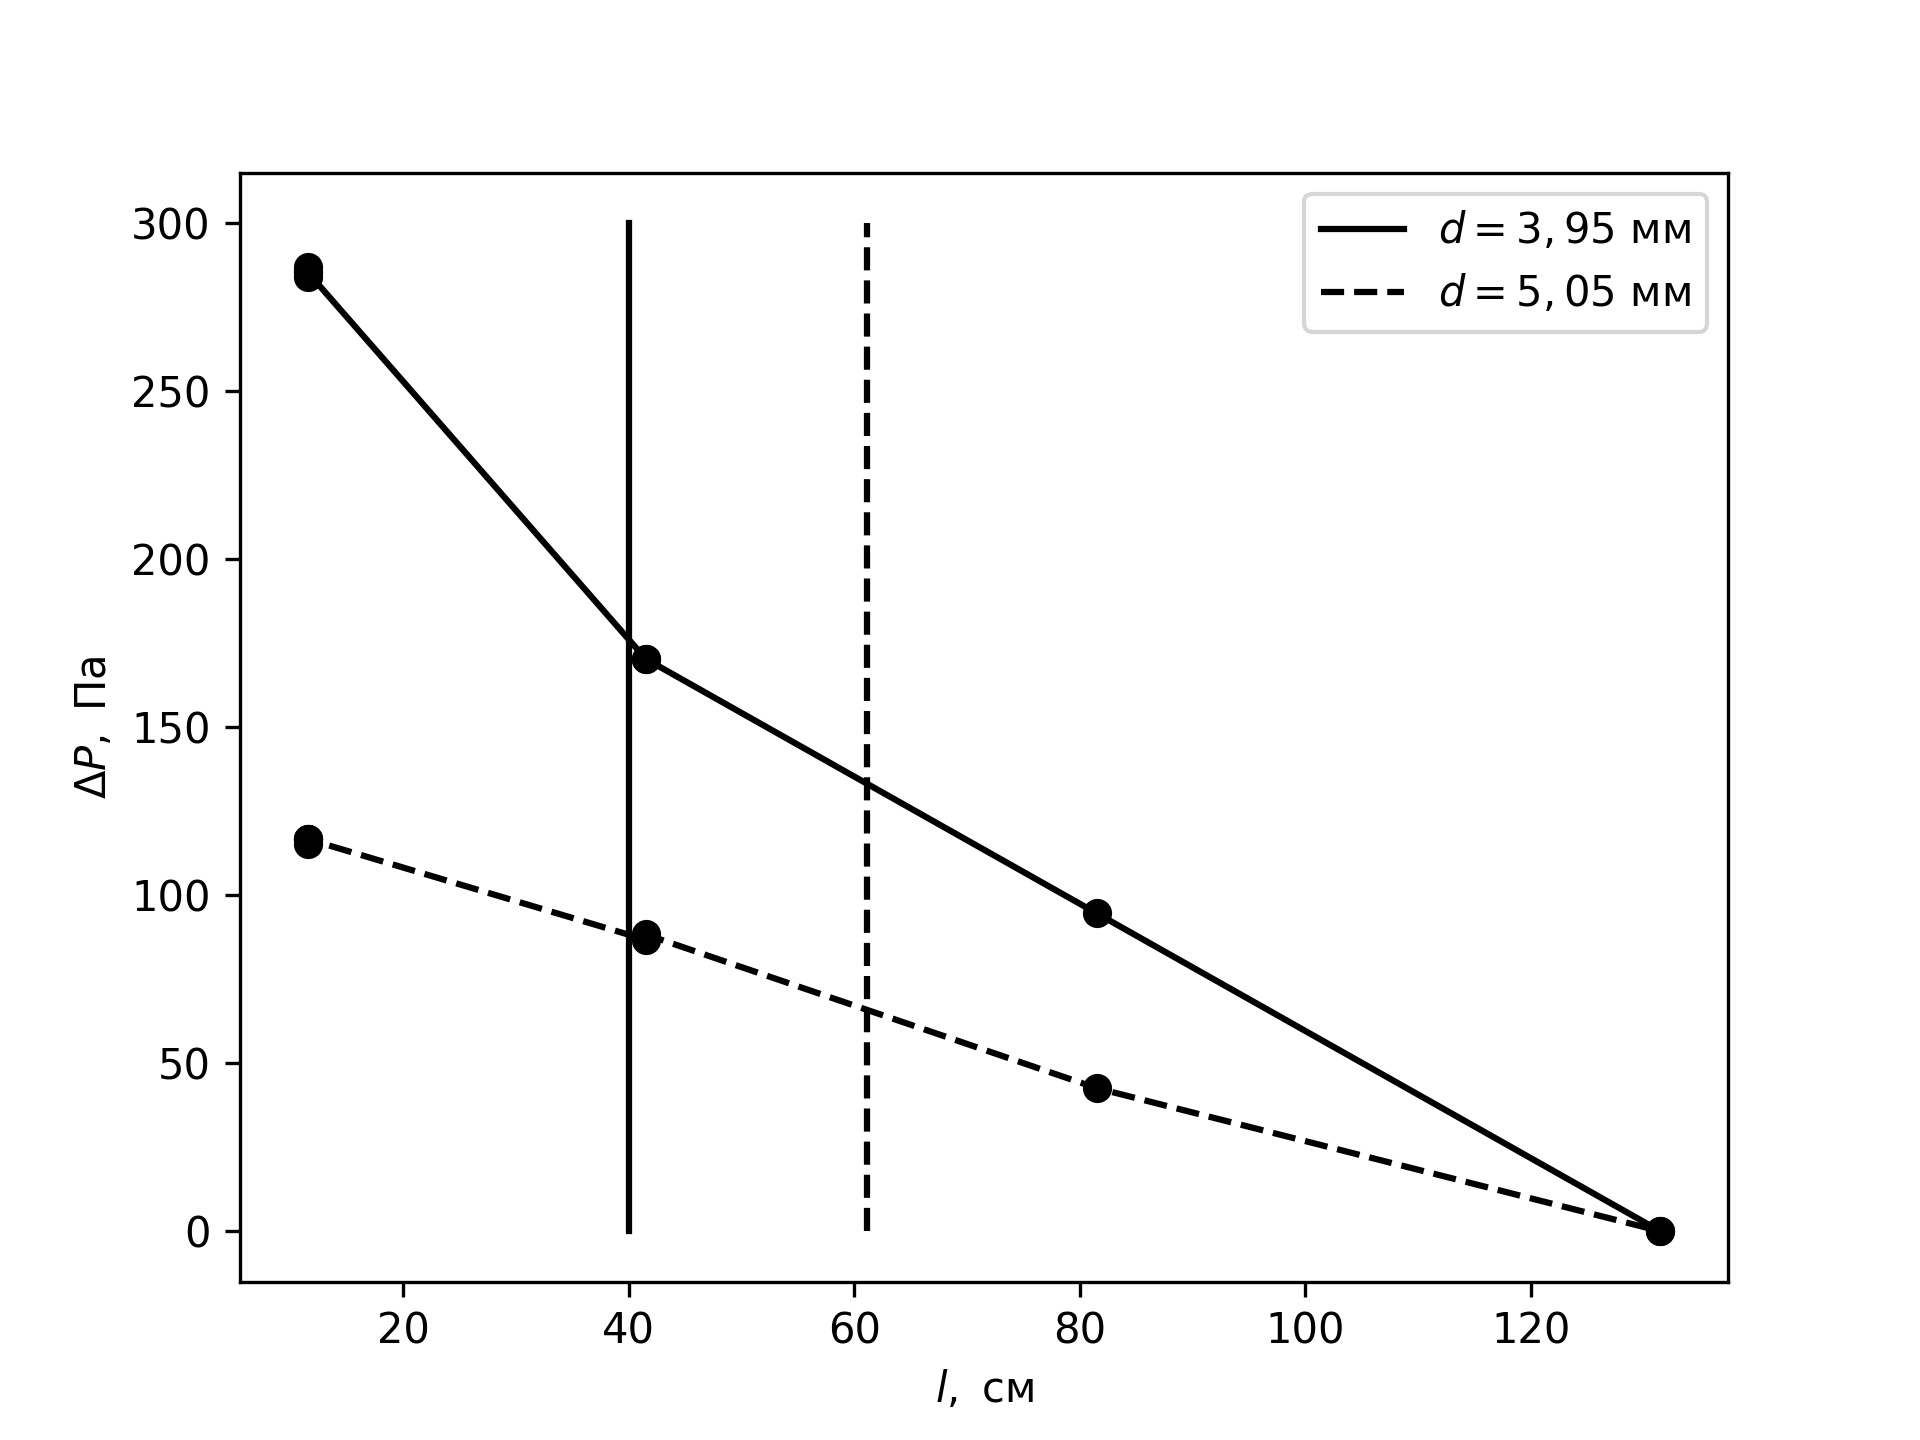
\includegraphics[width=0.8\linewidth]{terma3_2.png}
\caption{Распределение давления газа вдоль трубок}
\end{figure}

\begin{figure}[!ht]
\centering
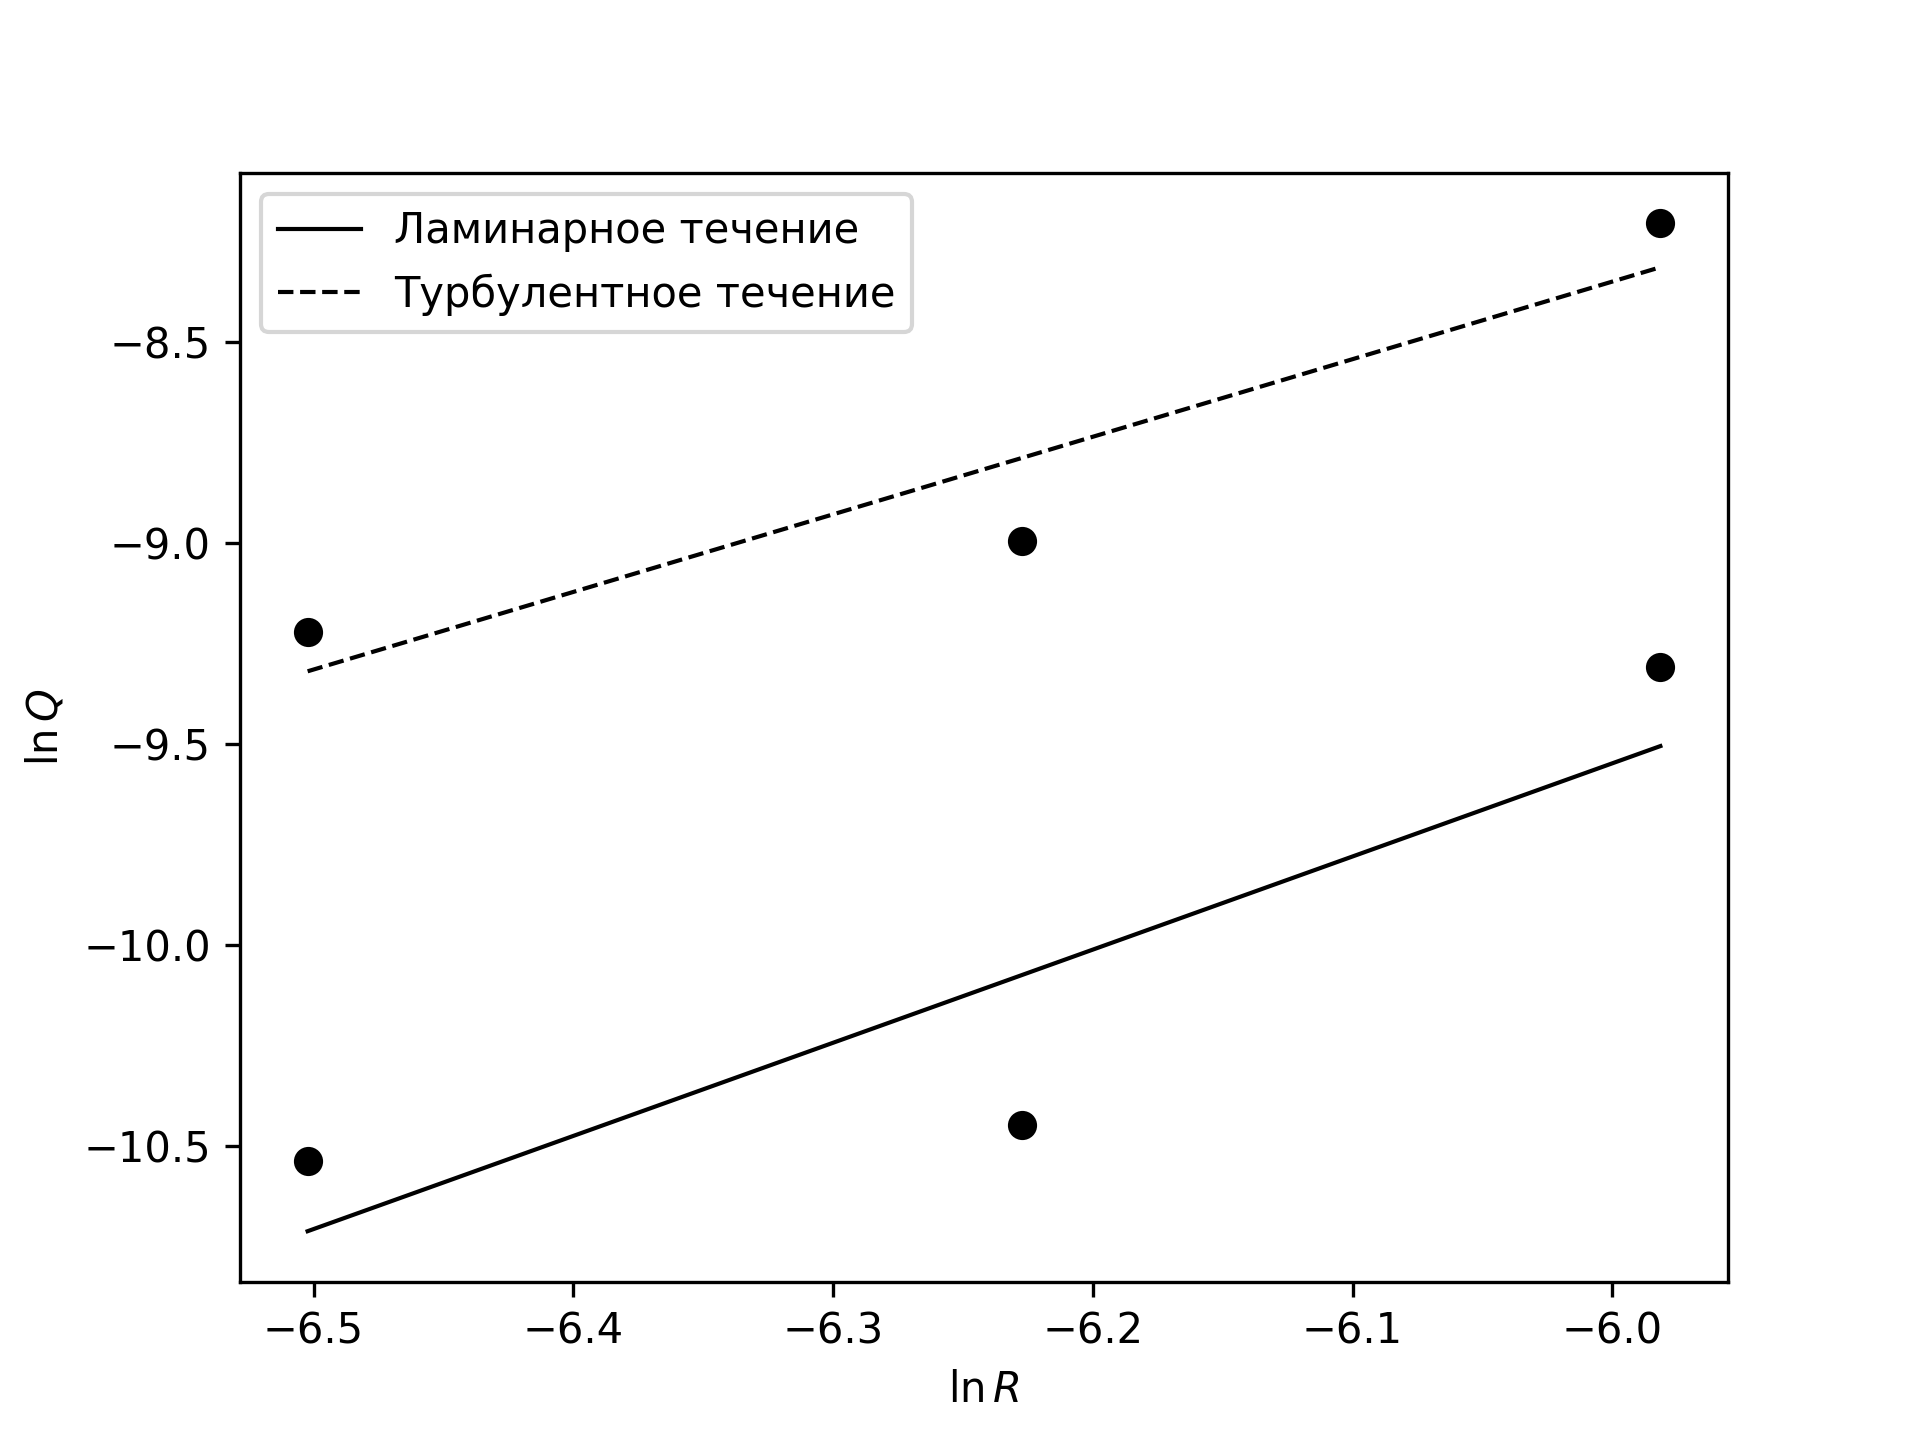
\includegraphics[width=0.8\linewidth]{terma3_3.png}
\caption{Зависимость $\ln Q(\ln R)$}
\end{figure}

\end{document}